\documentclass[11pt]{article}   	% use "amsart" instead of "article" for AMSLaTeX format
\usepackage{geometry}                		% See geometry.pdf to learn the layout options. There are lots.
\geometry{letterpaper}                   		% ... or a4paper or a5paper or ...
\geometry{landscape}                		% Activate for rotated page geometry
\geometry{left=5mm, top=20mm, right=5mm, bottom=30mm}
%\usepackage[parfill]{parskip}    		% Activate to begin paragraphs with an empty line rather than an indent
\usepackage{graphicx}				% Use pdf, png, jpg, or eps§ with pdflatex; use eps in DVI mode
								% TeX will automatically convert eps --> pdf in pdflatex
\usepackage{amssymb}
\usepackage{units}

%SetFonts


%SetFonts
\begin{document}
    \pagenumbering{gobble}
%\section{}
%\subsection{}
    \begin{figure}
        \begin{minipage}{0.49\textwidth}
            \centering
            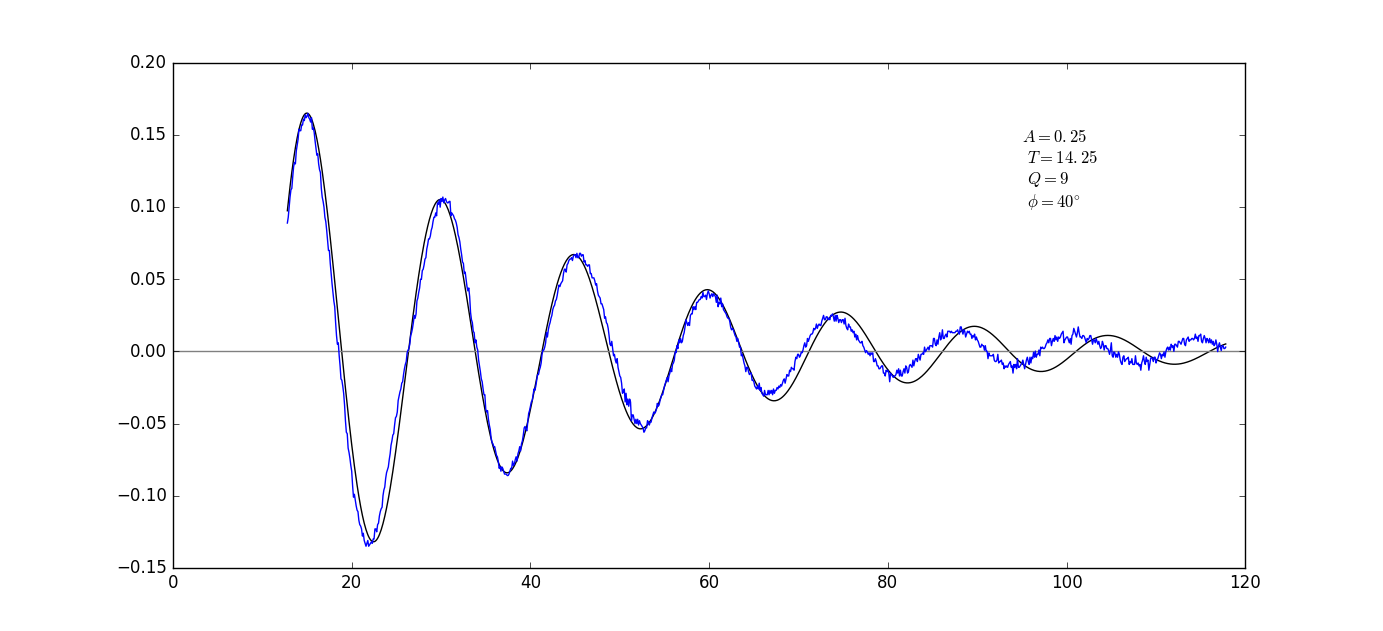
\includegraphics[width=1.1\textwidth]{blowfit.png}
            \caption{Seismometer Response Sans Magnet}
            \label{fig:nomag}
        \end{minipage}
        %
        \begin{minipage}{0.49\textwidth}
            \centering
            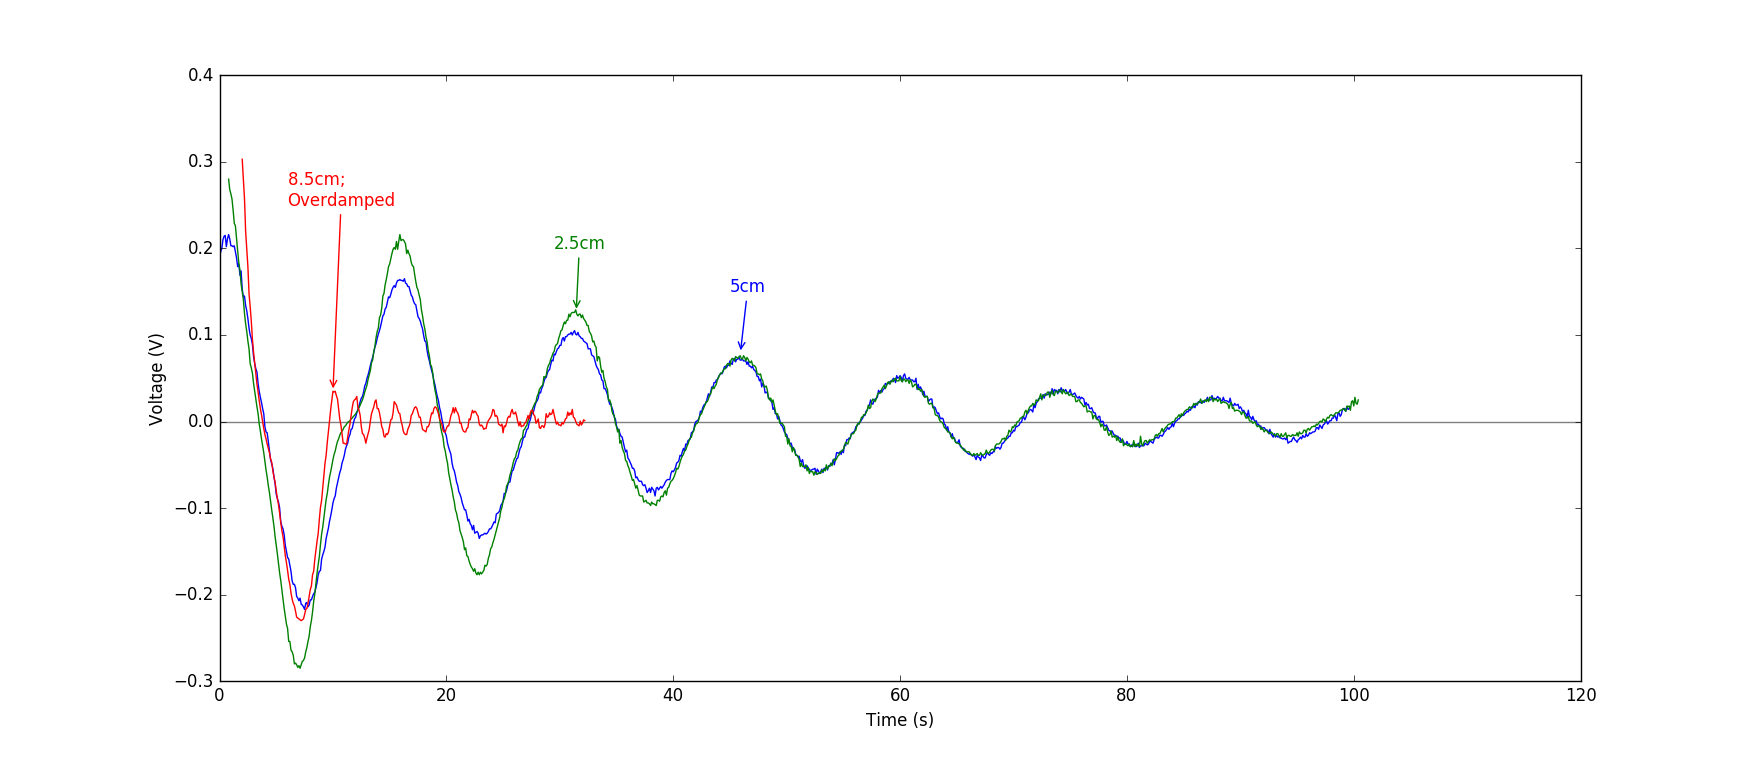
\includegraphics[width=1.1\textwidth]{3curvesbest.png}
            \caption{Oscillations for 3 Magnet Positions}
            \label{fig:3curves}
        \end{minipage}
    \end{figure}
    %
    \begin{figure}
        \begin{minipage}{0.49\textwidth}
            \centering
            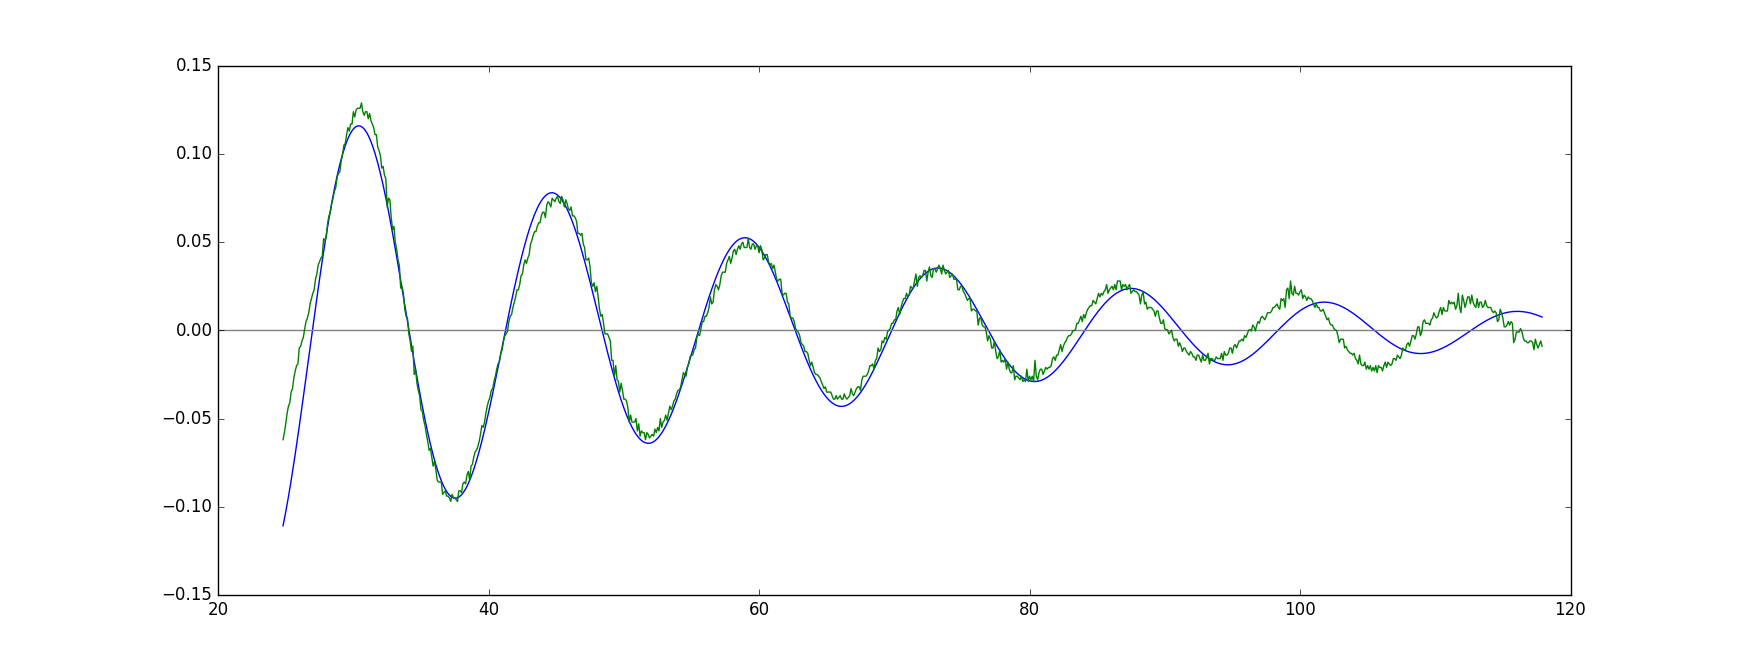
\includegraphics[width=1.1\textwidth]{blow5better.png}
            \caption{Oscillations with Magnet at $\unit[5]{cm}$}
            \label{fig:5cm}
        \end{minipage}
        %
        \begin{minipage}{0.49\textwidth}
            \centering
            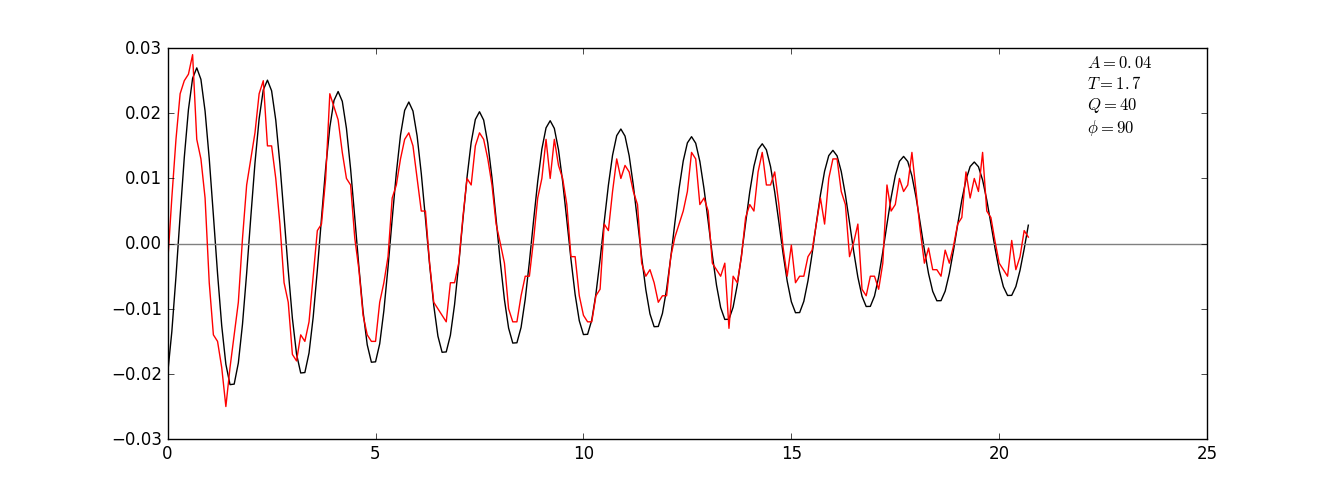
\includegraphics[width=1.1\textwidth]{overdampedmicrooscillations1.png}
            \caption{Overdamped Micro Oscillations}
            \label{fig:overdamped}
        \end{minipage}
    \end{figure}

\end{document}
